\documentclass[tikz,border=10pt]{standalone}
\usepackage{mathabx}
\usepackage{newunicodechar}
\newunicodechar{♮}{$\natural$}
\newunicodechar{♭}{$\flat$}
\newunicodechar{♯}{$\sharp$}
\newunicodechar{➚}{$\nearrow$}
\newunicodechar{➘}{$\searrow$}
\newunicodechar{Ȧ}{\stackon[0.8pt]{A}{.}}
\newunicodechar{Ḃ}{\stackon[0.8pt]{B}{.}}
\newunicodechar{Ċ}{\stackon[0.8pt]{C}{.}}
\newunicodechar{Ḋ}{\stackon[0.8pt]{D}{.}}
\newunicodechar{Ė}{\stackon[0.8pt]{E}{.}}
\newunicodechar{Ḟ}{\stackon[0.8pt]{F}{.}}
\newunicodechar{Ġ}{\stackon[0.8pt]{G}{.}}
\begin{document}
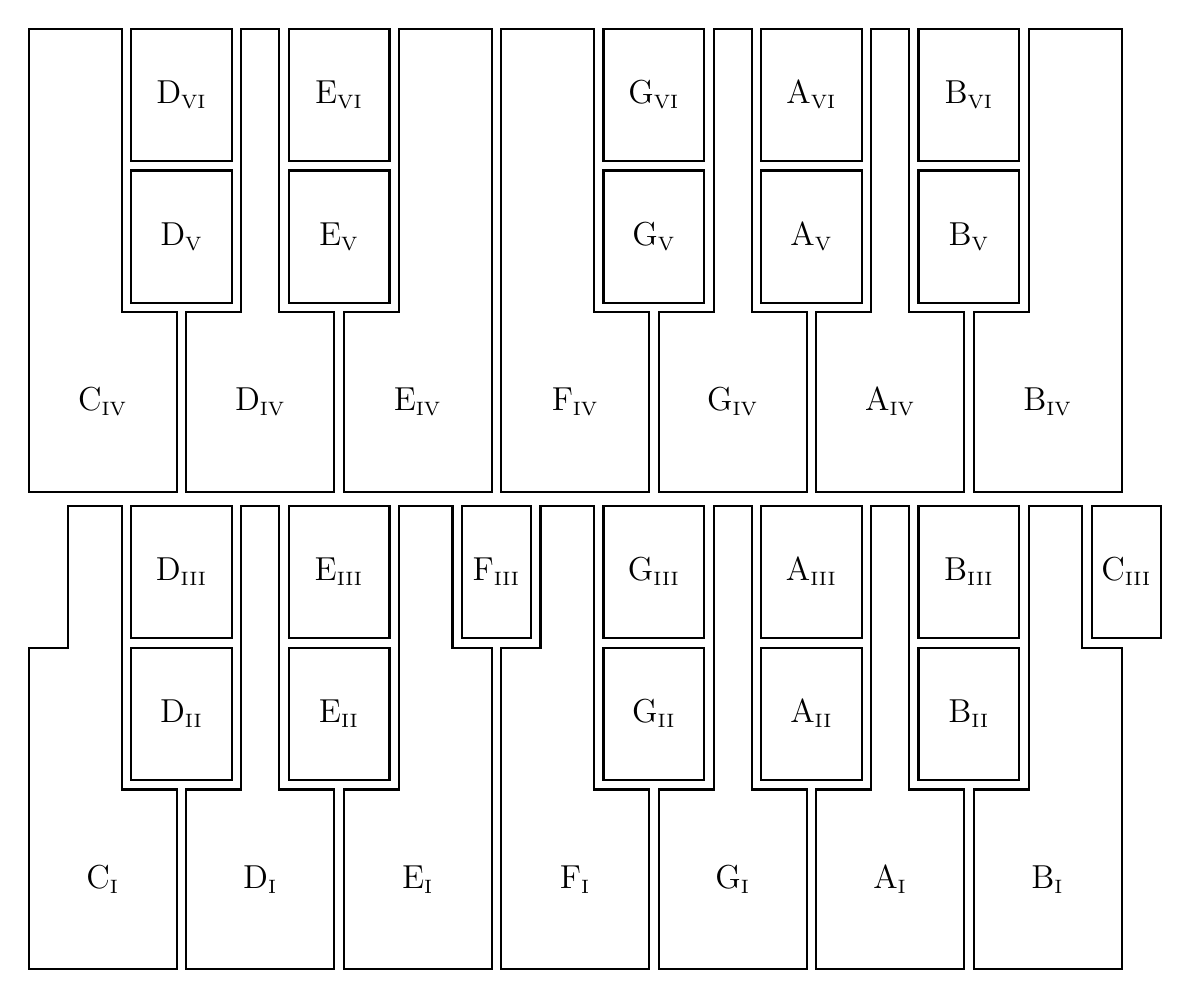
\begin{tikzpicture}

\draw[thick] (2.46, 2.46) -- (4.34, 2.46) -- (4.34, 4.7400002) -- (3.64, 4.7400002) -- (3.64, 8.34) -- (2.96, 8.34) -- (2.96, 6.5400004) -- (2.46, 6.5400004) --  cycle;
\draw[thick] (3.76, 4.86) -- (5.0400004, 4.86) -- (5.0400004, 6.5400004) -- (3.76, 6.5400004) --  cycle;
\draw[thick] (3.76, 6.66) -- (5.0400004, 6.66) -- (5.0400004, 8.34) -- (3.76, 8.34) --  cycle;
\draw[thick] (4.46, 2.46) -- (6.34, 2.46) -- (6.34, 4.7400002) -- (5.6400003, 4.7400002) -- (5.6400003, 8.34) -- (5.16, 8.34) -- (5.16, 4.7400002) -- (4.46, 4.7400002) --  cycle;
\draw[thick] (5.7599998, 4.86) -- (7.0400004, 4.86) -- (7.0400004, 6.5400004) -- (5.7599998, 6.5400004) --  cycle;
\draw[thick] (5.7599998, 6.66) -- (7.0400004, 6.66) -- (7.0400004, 8.34) -- (5.7599998, 8.34) --  cycle;
\draw[thick] (6.46, 2.46) -- (8.34, 2.46) -- (8.34, 6.5400004) -- (7.84, 6.5400004) -- (7.84, 8.34) -- (7.16, 8.34) -- (7.16, 4.7400002) -- (6.46, 4.7400002) --  cycle;
\draw[thick] (7.96, 6.66) -- (8.84, 6.66) -- (8.84, 8.34) -- (7.96, 8.34) --  cycle;
\draw[thick] (8.46, 2.46) -- (10.34, 2.46) -- (10.34, 4.7400002) -- (9.64, 4.7400002) -- (9.64, 8.34) -- (8.96, 8.34) -- (8.96, 6.5400004) -- (8.46, 6.5400004) --  cycle;
\draw[thick] (9.76, 4.86) -- (11.04, 4.86) -- (11.04, 6.5400004) -- (9.76, 6.5400004) --  cycle;
\draw[thick] (9.76, 6.66) -- (11.04, 6.66) -- (11.04, 8.34) -- (9.76, 8.34) --  cycle;
\draw[thick] (10.46, 2.46) -- (12.34, 2.46) -- (12.34, 4.7400002) -- (11.64, 4.7400002) -- (11.64, 8.34) -- (11.16, 8.34) -- (11.16, 4.7400002) -- (10.46, 4.7400002) --  cycle;
\draw[thick] (11.76, 4.86) -- (13.04, 4.86) -- (13.04, 6.5400004) -- (11.76, 6.5400004) --  cycle;
\draw[thick] (11.76, 6.66) -- (13.04, 6.66) -- (13.04, 8.34) -- (11.76, 8.34) --  cycle;
\draw[thick] (12.46, 2.46) -- (14.339999, 2.46) -- (14.339999, 4.7400002) -- (13.639999, 4.7400002) -- (13.639999, 8.34) -- (13.160001, 8.34) -- (13.160001, 4.7400002) -- (12.46, 4.7400002) --  cycle;
\draw[thick] (13.760001, 4.86) -- (15.04, 4.86) -- (15.04, 6.5400004) -- (13.760001, 6.5400004) --  cycle;
\draw[thick] (13.760001, 6.66) -- (15.04, 6.66) -- (15.04, 8.34) -- (13.760001, 8.34) --  cycle;
\draw[thick] (14.460001, 2.46) -- (16.34, 2.46) -- (16.34, 6.5400004) -- (15.839999, 6.5400004) -- (15.839999, 8.34) -- (15.160001, 8.34) -- (15.160001, 4.7400002) -- (14.460001, 4.7400002) --  cycle;
\draw[thick] (15.960001, 6.66) -- (16.84, 6.66) -- (16.84, 8.34) -- (15.960001, 8.34) --  cycle;
\draw[thick] (2.46, 8.5199995) -- (4.34, 8.5199995) -- (4.34, 10.8) -- (3.64, 10.8) -- (3.64, 14.400001) -- (2.46, 14.400001) --  cycle;
\draw[thick] (3.76, 10.92) -- (5.0400004, 10.92) -- (5.0400004, 12.6) -- (3.76, 12.6) --  cycle;
\draw[thick] (3.76, 12.72) -- (5.0400004, 12.72) -- (5.0400004, 14.400001) -- (3.76, 14.400001) --  cycle;
\draw[thick] (4.46, 8.5199995) -- (6.34, 8.5199995) -- (6.34, 10.8) -- (5.6400003, 10.8) -- (5.6400003, 14.400001) -- (5.16, 14.400001) -- (5.16, 10.8) -- (4.46, 10.8) --  cycle;
\draw[thick] (5.7599998, 10.92) -- (7.0400004, 10.92) -- (7.0400004, 12.6) -- (5.7599998, 12.6) --  cycle;
\draw[thick] (5.7599998, 12.72) -- (7.0400004, 12.72) -- (7.0400004, 14.400001) -- (5.7599998, 14.400001) --  cycle;
\draw[thick] (6.46, 8.5199995) -- (8.34, 8.5199995) -- (8.34, 14.400001) -- (7.16, 14.400001) -- (7.16, 10.8) -- (6.46, 10.8) --  cycle;
\draw[thick] (8.46, 8.5199995) -- (10.34, 8.5199995) -- (10.34, 10.8) -- (9.64, 10.8) -- (9.64, 14.400001) -- (8.46, 14.400001) --  cycle;
\draw[thick] (9.76, 10.92) -- (11.04, 10.92) -- (11.04, 12.6) -- (9.76, 12.6) --  cycle;
\draw[thick] (9.76, 12.72) -- (11.04, 12.72) -- (11.04, 14.400001) -- (9.76, 14.400001) --  cycle;
\draw[thick] (10.46, 8.5199995) -- (12.34, 8.5199995) -- (12.34, 10.8) -- (11.64, 10.8) -- (11.64, 14.400001) -- (11.16, 14.400001) -- (11.16, 10.8) -- (10.46, 10.8) --  cycle;
\draw[thick] (11.76, 10.92) -- (13.04, 10.92) -- (13.04, 12.6) -- (11.76, 12.6) --  cycle;
\draw[thick] (11.76, 12.72) -- (13.04, 12.72) -- (13.04, 14.400001) -- (11.76, 14.400001) --  cycle;
\draw[thick] (12.46, 8.5199995) -- (14.339999, 8.5199995) -- (14.339999, 10.8) -- (13.639999, 10.8) -- (13.639999, 14.400001) -- (13.160001, 14.400001) -- (13.160001, 10.8) -- (12.46, 10.8) --  cycle;
\draw[thick] (13.760001, 10.92) -- (15.04, 10.92) -- (15.04, 12.6) -- (13.760001, 12.6) --  cycle;
\draw[thick] (13.760001, 12.72) -- (15.04, 12.72) -- (15.04, 14.400001) -- (13.760001, 14.400001) --  cycle;
\draw[thick] (14.460001, 8.5199995) -- (16.34, 8.5199995) -- (16.34, 14.400001) -- (15.160001, 14.400001) -- (15.160001, 10.8) -- (14.460001, 10.8) --  cycle;
\node at (3.4, 3.6000001) { \large C\textsubscript{\scriptsize I} };
\node at (5.4, 3.6000001) { \large D\textsubscript{\scriptsize I} };
\node at (7.4, 3.6000001) { \large E\textsubscript{\scriptsize I} };
\node at (9.400001, 3.6000001) { \large F\textsubscript{\scriptsize I} };
\node at (11.400001, 3.6000001) { \large G\textsubscript{\scriptsize I} };
\node at (13.400001, 3.6000001) { \large A\textsubscript{\scriptsize I} };
\node at (15.400001, 3.6000001) { \large B\textsubscript{\scriptsize I} };
\node at (4.4, 5.7000003) { \large D\textsubscript{\scriptsize II} };
\node at (6.4, 5.7000003) { \large E\textsubscript{\scriptsize II} };
\node at (10.400001, 5.7000003) { \large G\textsubscript{\scriptsize II} };
\node at (12.400001, 5.7000003) { \large A\textsubscript{\scriptsize II} };
\node at (14.400001, 5.7000003) { \large B\textsubscript{\scriptsize II} };
\node at (4.4, 7.5) { \large D\textsubscript{\scriptsize III} };
\node at (6.4, 7.5) { \large E\textsubscript{\scriptsize III} };
\node at (10.400001, 7.5) { \large G\textsubscript{\scriptsize III} };
\node at (12.400001, 7.5) { \large A\textsubscript{\scriptsize III} };
\node at (14.400001, 7.5) { \large B\textsubscript{\scriptsize III} };
\node at (8.400001, 7.5) { \large F\textsubscript{\scriptsize III} };
\node at (16.4, 7.5) { \large C\textsubscript{\scriptsize III} };
\node at (3.4, 9.66) { \large C\textsubscript{\scriptsize IV} };
\node at (5.4, 9.66) { \large D\textsubscript{\scriptsize IV} };
\node at (7.4, 9.66) { \large E\textsubscript{\scriptsize IV} };
\node at (9.400001, 9.66) { \large F\textsubscript{\scriptsize IV} };
\node at (11.400001, 9.66) { \large G\textsubscript{\scriptsize IV} };
\node at (13.400001, 9.66) { \large A\textsubscript{\scriptsize IV} };
\node at (15.400001, 9.66) { \large B\textsubscript{\scriptsize IV} };
\node at (4.4, 11.76) { \large D\textsubscript{\scriptsize V} };
\node at (6.4, 11.76) { \large E\textsubscript{\scriptsize V} };
\node at (10.400001, 11.76) { \large G\textsubscript{\scriptsize V} };
\node at (12.400001, 11.76) { \large A\textsubscript{\scriptsize V} };
\node at (14.400001, 11.76) { \large B\textsubscript{\scriptsize V} };
\node at (4.4, 13.56) { \large D\textsubscript{\scriptsize VI} };
\node at (6.4, 13.56) { \large E\textsubscript{\scriptsize VI} };
\node at (10.400001, 13.56) { \large G\textsubscript{\scriptsize VI} };
\node at (12.400001, 13.56) { \large A\textsubscript{\scriptsize VI} };
\node at (14.400001, 13.56) { \large B\textsubscript{\scriptsize VI} };
\end{tikzpicture}
\end{document}